\documentclass{standalone}
 
% Required package
\usepackage{tikz}
\usepackage{amssymb}
\usepackage{ntheorem}
\usepackage{tensor}
%\usepackage{physics}
\usepackage[italicdiff]{physics}
\usepackage{calc}
\usepackage{mathrsfs}
 \usetikzlibrary {backgrounds,mindmap}
 \usetikzlibrary{decorations.pathmorphing,decorations.markings}
\usetikzlibrary{decorations.pathreplacing} %
\begin{document}
 
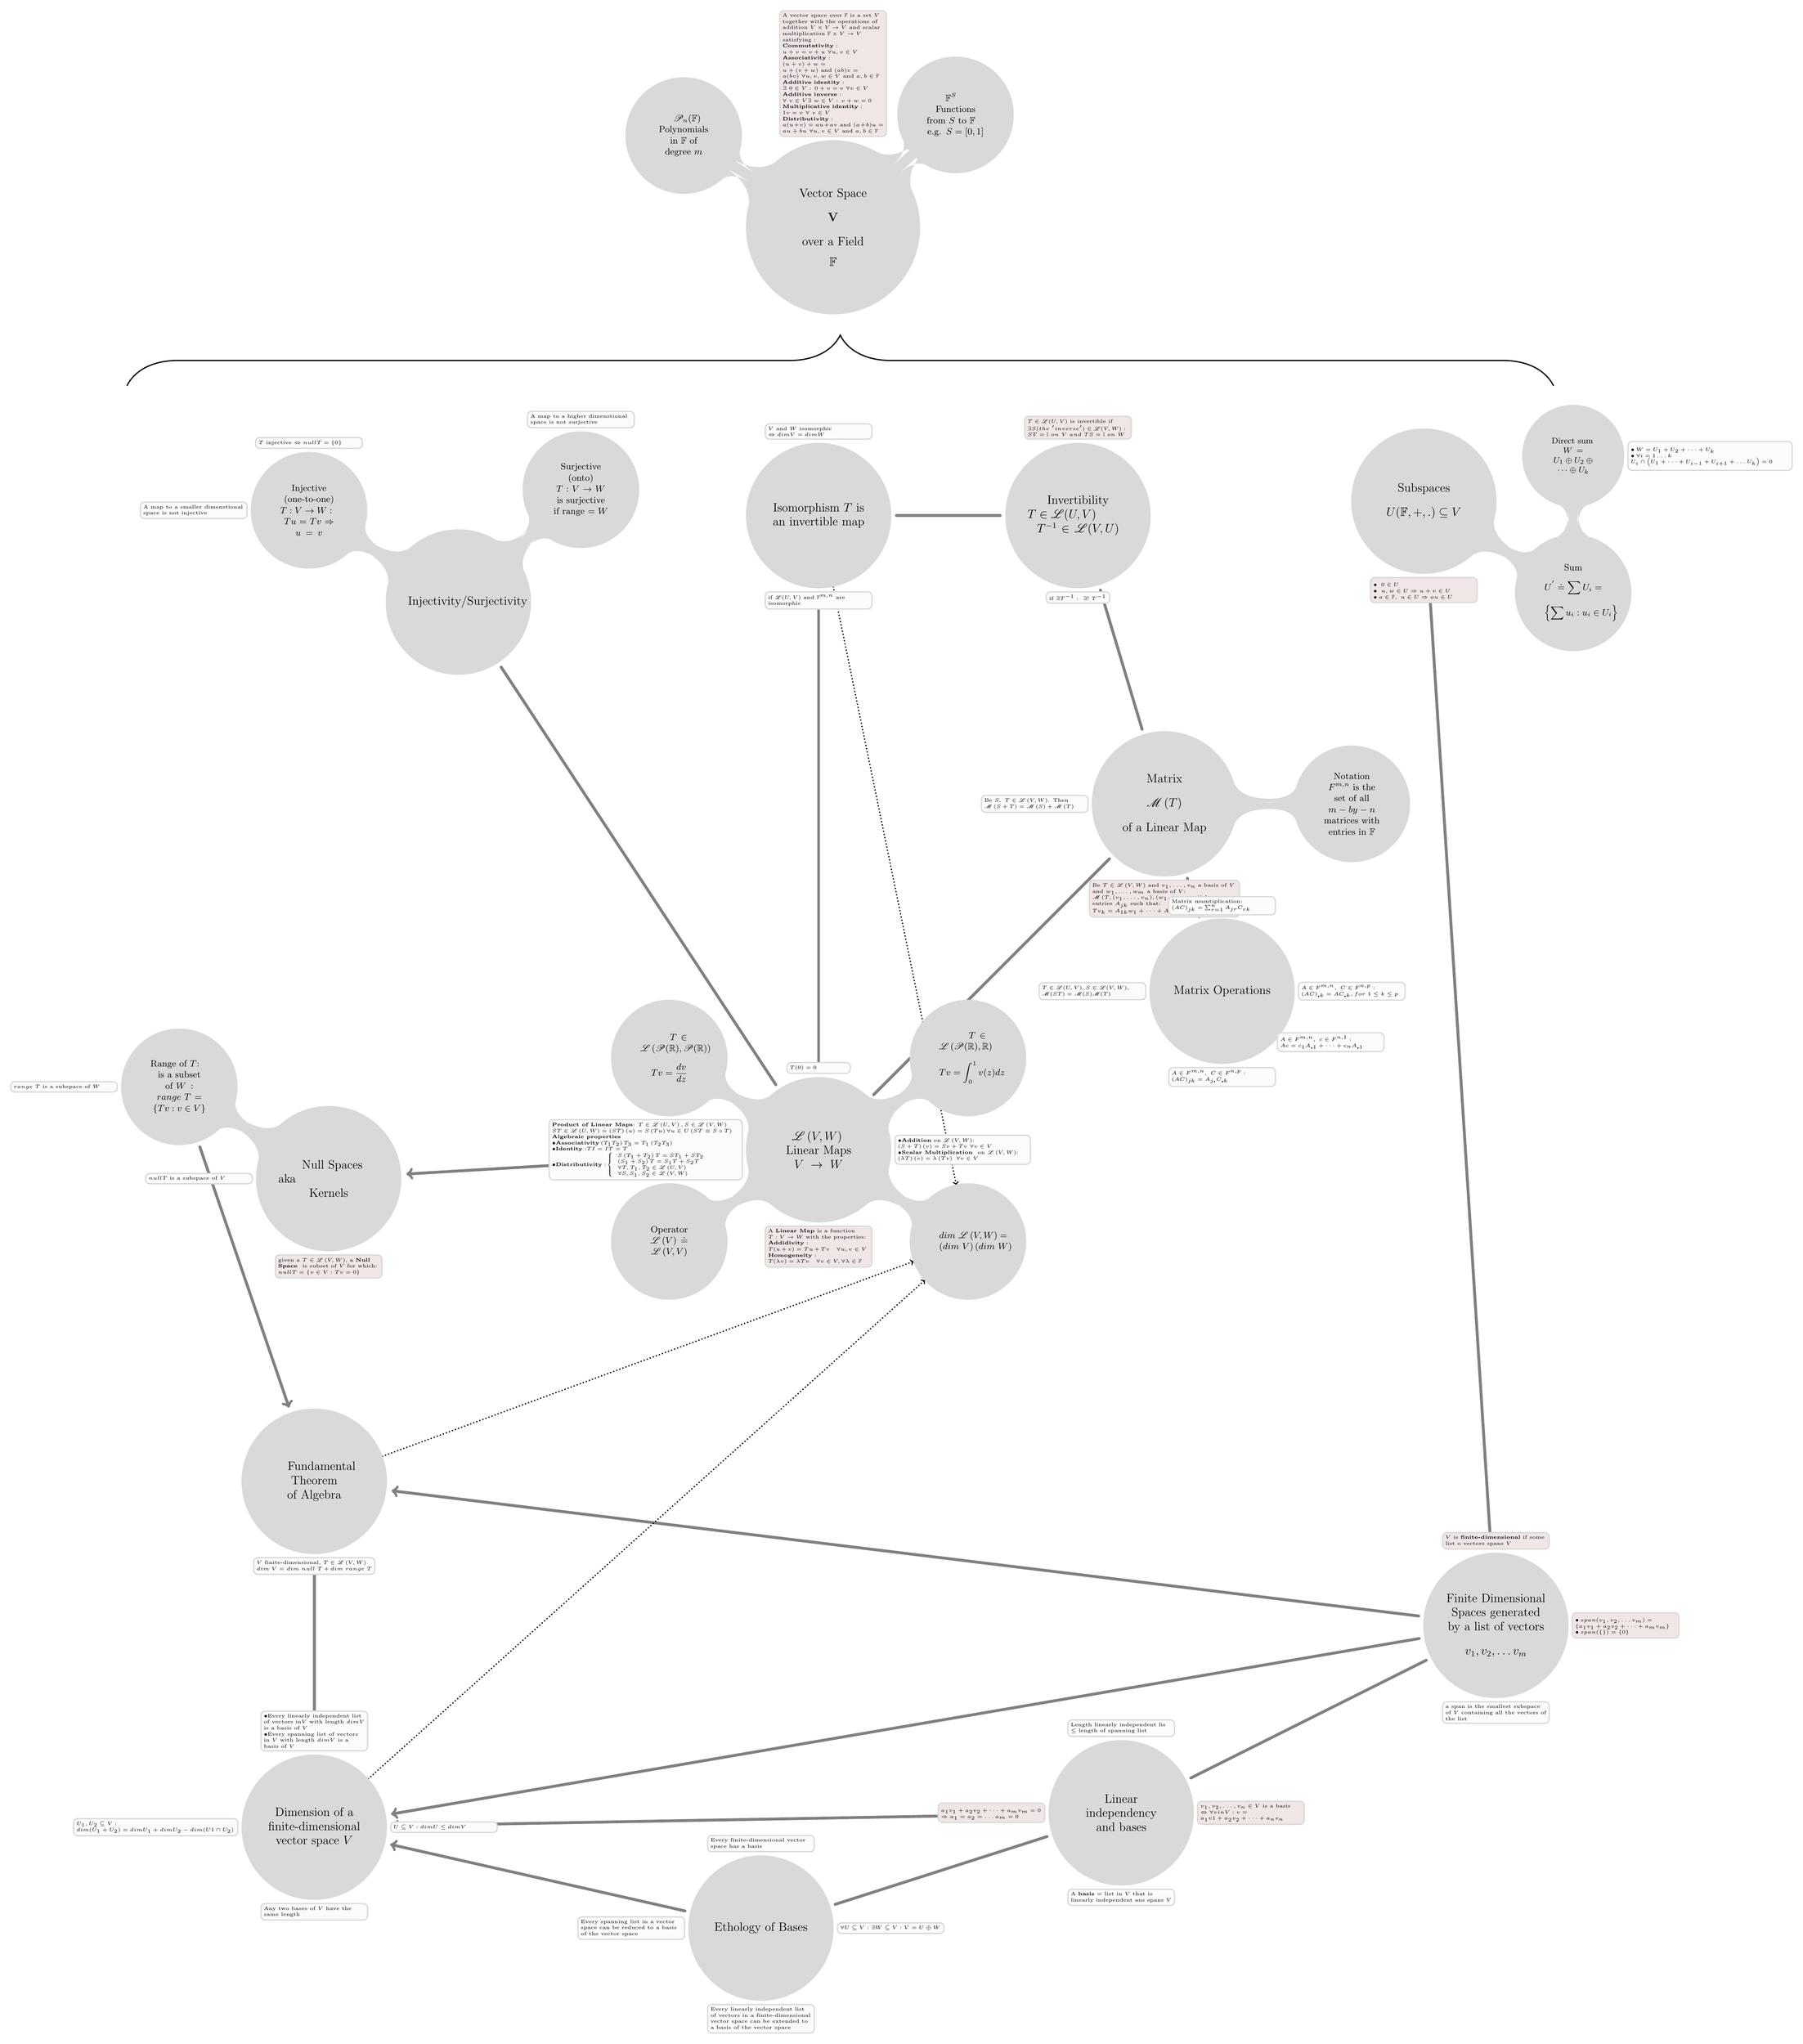
\begin{tikzpicture}[
    mindmap,
    concept color = gray!30,
    every node/.style = {concept},
    grow cyclic,
    minimum size=5cm,
    every annotation/.style={fill=gray!3},
    level 1/.append style = {
        concept color = gray!30,
        minimum size=4cm,
        level distance = 4.5cm,
        sibling angle = 120
    },
    level 2/.append style = {
        concept color = gray!30,
        minimum size=3.5cm,
        level distance = 3cm,
        sibling angle = 45
    }
]
\definecolor{def}{RGB}{240,230,230}
 
\coordinate(N1) at (-24.5,65.5) {} {} {} ;
\coordinate(N2) at (-4,56) {};
\coordinate(N3) at (-1.5,17) {} {} ;
\coordinate(N4) at (-14.5,10.5) {} {};
\coordinate(N5) at (-27,6.5) {};
\coordinate(N6) at (-42.5,10);
\coordinate(N7) at (-25,33.5) {} {} ;
\coordinate(N8) at (-42,32.5) {} {} ;
\coordinate(N9) at (-37.5,52.5) ;
\coordinate(N10) at (-42.5,22) ;
\coordinate(N11) at (-13,45.5) {} {} {} ;
\coordinate(N12) at (-11,39) {} {} {};
\coordinate(N13) at (-16,55.5) {} ;
\coordinate(N14) at (-25,55.5) {};
%%Vector spaces
\node (VS) [concept,minimum size=6cm]
 at (N1){Vector Space $$\mathbf{V}$$ $$\text{over a Field}$$$$\mathbb{F}$$}
child [grow = north west]{node[left](VS2)  {$\quad\quad \mathscr{P}_n(\mathbb{F})$ \newline  Polynomials in $\mathbb{F}$ of degree $m$}}
child {node[right](VS2)   {$\quad\quad \mathbb{F}^S$ \newline Functions from $S$ to $\mathbb{F}$\newline e.g. $S=[0,1]$}};
  \node [annotation,above,, fill=def] at (VS.north){A  vector space  over $\mathbb{F}$ is a set $V$ together with the operations of addition $V \times V \to V$ and scalar multiplication $\mathbb{F} \times V \to V$ satisfying :
$ \newline \mathbf{Commutativity: } \newline u+v=v+u \ \forall u,v\in V$
$ \newline\mathbf{Associativity: } \newline (u+v)+w= u+(v+w) \text{ and }  (ab) v = a(bv) \ \forall u,v,w\in V \text{ and }  a,b\in \mathbb{F}$ 
$ \newline \mathbf{Additive \ identity: }  \newline \exists \ 0\in V$ : $0+v=v\ \forall v\in V$
$ \newline \mathbf{Additive \ inverse : }   \newline\forall \ v\in V \exists  \ w\in V$ : $v+w=0$
$ \newline \mathbf{Multiplicative \ identity: }  \newline  1v=v\  \forall \ v\in V$
$ \newline \mathbf{Distributivity: } \newline  a(u+v)=au+av \text{ and } (a+b)u=au+bu\  \forall u,v\in V \text{ and } a,b\in\mathbb{F}$  };

\draw [decorate, decoration={brace, amplitude=50pt}](-49,60)--(0.5,60);
%%Subspaces
 \node (Subsp) at (N2){Subspaces $$ U(\mathbb{F},+,.) \subseteq V$$ }
    child [grow =south east] {node[right](sum) {Sum $$U^{'}\doteq \sum U_i = $$ $$\left\{ \sum u_i : u_i \in  U_i \right\}$$}
	child [grow = north ] {node [above](dsum) {Direct sum \newline $W=  U_1\oplus U_2 \oplus \dots \oplus U_k$}} };
 \node [annotation,below, fill=def] at (Subsp.south){
$ \newline \bullet \ 0 \in U$
$\newline  \bullet \ u,w \in U \Rightarrow u+v \in U$ 
$\newline  \bullet  a \in \mathbb{F},  \  u \in U \Rightarrow au \in U$  };
\node [annotation,minimum width=5.5cm, minimum height=1cm,right,text width=5.5cm] at (dsum.east){
$ \newline \bullet W= U_1+ U_2 + \dots +U_k $
$\newline \bullet \forall i=1 \dots k$
$\newline   \quad U_i \cap  \left(U_1+\dots +U_{i-1}+U_{i+1}+\dots  U_k\right) = {0}$
};

 %%Finite Dimensional Spaces generated by a list of vectors
 \node[] (FDS) at (N3){Finite Dimensional Spaces generated by a list of vectors$$v_1,v_2,\dots v_m$$ };
 \node [annotation,right, fill=def] at (FDS.east){$\newline \bullet span(v_1,v_2,\dots v_m)=\left\{ a_1v_1+a_2v_2+\dots +a_mv_m\right\}\newline \bullet span(\{\})= \{0\}$};
 \node [annotation,below] at (FDS.south){a span is the smallest subspace of $V$ containing all the vectors of the list};
\node [annotation, above, fill=def] at (FDS.north){$V$ is $\textbf{finite-dimensional}$ if some list o vectors spans $V$ };

%%Linear independency
\node (LI) at (N4){Linear\\ independency and bases };
\node [annotation, left, fill=def] at (LI.west){$\newline a_1v_1+ a_2v_2+\dots +a_mv_m=0 \newline \Rightarrow a_1=a_2=\dots  a_m=0$ };
\node [annotation, above] at (LI.north){Length linearly independent lis $\le$ length of spanning list};
\node [annotation, below] at (LI.south){A \textbf{basis} $=$ list in $V$ that is linearly independent ans spans $V$};
\node [annotation,right, fill=def] at (LI.east){ $v_1, v_2, \dots, v_n \in V$ is a basis $\Leftrightarrow \forall v in V: v=a_1v1+a_2v_2+\dots +a_nv_n$};

%%Bases
\node (Bases) at (N5){Ethology of Bases  };
\node [annotation, left] at (Bases.west){Every spanning list in a vector space can be reduced to a basis of the vector space };
\node [annotation, above] at (Bases.north){Every finite-dimensional vector space has a basis};
\node [annotation, below] at (Bases.south){Every linearly independent list of vectors in a finite-dimensional vector space can be extended to a basis of the vector space};
\node [annotation,right] at (Bases.east){ $\forall U \subseteq V: \exists W \subseteq V: V=U\oplus W$};

%%Dimension af a vector space
\node (Dim) at (N6){Dimension of a finite-dimensional  vector space $V$ };
\node [annotation, below] at (Dim.south){Any two bases of $V$ have the same length };
\node [annotation, right] at (Dim.east){$U\subseteq V: dim U \leq dim V$ };
\node [annotation,above] at (Dim.north){$\bullet$Every linearly independent list of vectors in$V$ with length $dim V$ is a basis of $V$
\newline $\bullet$Every spanning list of vectors in $V$ with length $dim V$ is a basis of $V$};
\node [annotation,left,minimum width=5.5cm,text width=5.5cm] at (Dim.west){$U_1,U_2 \subseteq V: \newline dim (U_1+U_2)=dim U_1+dim U_2-dim (U1\cap U_2)$ };


%%Linear Maps
\node (LM) at (N7){$  \quad\quad\mathscr{L}\left(V,W\right)$ \newline Linear Maps  $V\rightarrow W$ }
child [grow = north west]{node[left](LM1)  {$\quad\quad T\in \mathscr{L}\left(\mathscr{P(\mathbb{R}}),\mathscr{P(\mathbb{R}})\right)$ \newline $$Tv=\dv{v}{z}$$}}
child [grow = north east] {node[right](LM2)   {$\quad\quad T\in \mathscr{L}\left(\mathscr{P(\mathbb{R}}),\mathbb{R}\right)$ \newline $$Tv=\int_0^1 v(z)dz$$}}
child [grow = south east]{node[right](LM3)   {$dim \ \mathscr{L}\left(V,W\right) = \left(dim \  V\right)\left(dim \ W\right)$}}
child [grow = south west]{node[left](LM4)   {Operator $\mathscr{L}\left(V\right)\doteq \mathscr{L}\left(V,V\right)$}};
\node [annotation,below, fill=def] at (LM.south){A \textbf{Linear Map} is a function  $T:V\rightarrow W$  with the properties:
$ \newline \mathbf{Addidivity: } \newline T(u+v)=Tu+Tv \quad \forall u,v\in V$
$ \newline\mathbf{Homogeneity: } \newline T(\lambda v)= \lambda Tv \quad \forall v \in V , \forall \lambda \in \mathbb{F}$  };

\node [annotation, right,minimum width=4.5cm,text width=4.5cm] at (LM.east){$ \bullet$\textbf{Addition} on $\mathscr{L}\left(V,W\right)$:  $\left(S+T\right)(v)= Sv+Tv \ \forall v \in V$
\newline $ \bullet$\textbf{Scalar Multiplication } on $\mathscr{L}\left(V,W\right)$:  $\left(\lambda T\right)(v)= \lambda \left(Tv \right)\ \forall v \in V$};
\node [annotation,left,minimum width=6.5cm,text width=6.5cm] at (LM.west){\textbf{Product of Linear Maps}: $T\in \mathscr{L}\left(U,V\right), S\in \mathscr{L}\left(V,W\right)$ \newline
$ST \in\mathscr{L}\left(U,W\right)\doteq \left(ST\right)(u)= S\left(Tu\right) \forall u \in U \left(  ST \equiv S\circ T  \right) $ 
\newline \textbf{Algebraic properties  } 
\newline $ \quad\quad \bullet \mathbf{Associativity  } \left(T_1T_2\right)T_3= T_1\left(T_2T_3\right)$
\newline$\quad\quad \bullet\mathbf{Identity: } TI = IT = T$
\newline$\quad\quad \bullet\mathbf{Distributivity: } \left\{\begin{array}{l}S\left(T_1+T_2\right)T= ST_1+ST_2 \\ \left(S_1+S_2\right)T= S_1T+S_2T \\ \forall T,T_1,T_2 \in \mathscr{L}\left(U,V\right) \\  \forall S,S_1,S_2 \in \mathscr{L}\left(V,W\right)\end{array} \right.$};
\node [annotation, above ,text width=2.cm] at (LM.north){$ T(0)=0$};


%%Null Spaces 
\node (NS) at (N8){$\quad\quad$Null Spaces \newline $\quad\quad$ aka\newline Kernels  }
child [grow = north west]{node[left](NS1)  {Range  of $T$: \newline is a subset of $W: $ $range\ T=\left\{Tv: v\in V\right\}$}};
\node [annotation,below,fill=def] at (NS.south){given a $T\in \mathscr{L}\left(V,W\right)$, a  \textbf{Null Space }  is subset of $V$ for which:
\newline $ null T=\left \{v\in V: Tv=0\right\}$};
\node [annotation,left] at (NS.west){$nullT$ is a subspace of $V$};
\node [annotation,left] at (NS1.west){$range\ T$ is a subspace of $W$};

%%Injectivity/Surjectivity
\node (SI) at (N9){Injectivity/Surjectivity  }
child [grow = north west]{node[left](SI1)  {Injective (one-to-one) $ T:V\rightarrow W: \newline Tu=Tv \Rightarrow u=v $}}
child {node[right](SI2)   {Surjective (onto) $ T:V\rightarrow W$ is surjective if range $=W$ }};
\node [annotation,above] at (SI1.north){$T$ injective $\Leftrightarrow null T = \left\{ 0 \right\}$};
\node [annotation,left] at (SI1.west){A map to a smaller dimenstional space is not injective};
\node [annotation,above] at (SI2.north){A map to a higher dimenstional space is not surjective};
%%Fundamental Theorem of Algebra
\node (FTA) at (N10){$\quad \quad$Fundamental \newline Theorem of Algebra };
\node [annotation,below,text width=4.cm] at (FTA.south){$V$ finite-dimensional, $T \in \mathscr{L}\left(V,W\right)$
\newline $dim\ V = dim \ null \ T + dim \ range \ T$};

%%Injectivity/Surjectivity
\node (SI) at (N9){Injectivity/Surjectivity  }
child [grow = north west]{node[left](SI1)  {Injective (one-to-one) $ T:V\rightarrow W: \newline Tu=Tv \Rightarrow u=v $}}
child {node[right](SI2)   {Surjective (onto) $ T:V\rightarrow W$ is surjective if range $=W$ }};
\node [annotation,above] at (SI1.north){$T$ injective $\Leftrightarrow null T = \left\{ 0 \right\}$};
\node [annotation,left] at (SI1.west){A map to a smaller dimenstional space is not injective};
\node [annotation,above] at (SI2.north){A map to a higher dimenstional space is not surjective};


%%Fundamental Theorem of Algebra
\node (FTA) at (N10){$\quad \quad$Fundamental \newline Theorem of Algebra };
\node [annotation,below,text width=4.cm] at (FTA.south){$V$ finite-dimensional, $T \in \mathscr{L}\left(V,W\right)$
\newline $dim\ V = dim \ null \ T + dim \ range \ T$};

%%Matrices
\node (Mat) at (N11){Matrix $$\mathscr{M}\left(T\right)$$ of a Linear Map}
child {node[right](Mat1)   {Notation $ F^{m,n}$ is the set of all $m-by-n$ matrices with entries in $\mathbb{F}$}};
\node [annotation,below,text width=5.cm, fill=def] at (Mat.south){Be $T \in \mathscr{L}\left(V,W\right)$  and $v_1,\dots,v_n$ a basis of $V$ and $w_1,\dots,w_m$ a basis of $V$:\newline 
$\mathscr{M}\left(T,(v_1,\dots,v_n),(w_1,\dots,w_m)\right)$ has entries $A_{jk}$ such that:\newline
$Tv_k = A_{1k}w_1+\dots + A_{mk}w_m$};
\node [annotation,left,] at (Mat.west){Be $S, \ T \in \mathscr{L}\left(V,W\right)$. Then $\mathscr{M}\left(S+T\right)=\mathscr{M}\left(S\right)+\mathscr{M}\left(T\right)$ };
%\node [annotation,above] at (Mat.north){Matrix mumtiplication: $\left(AC\right)_{jk} = \sum_{r=1}^{n} A_{jr}C_{rk}$};

%%Operations with Matrices
\node (MatOp) at (N12){Matrix Operations};
\node [annotation,left,] at (MatOp.west){$T \in \mathscr{L}(U,V), S\in \mathscr{L}(V,W),$\newline
$ \mathscr{M}(ST)=\mathscr{M}(S)\mathscr{M}(T)$ };
\node [annotation,above] at (MatOp.north){Matrix mumtiplication: $\left(AC\right)_{jk} = \sum_{r=1}^{n} A_{jr}C_{rk}$};
\node [annotation,below] at (MatOp.south){$A \in F^{m,n},\ C \in F^{n,p}:\ \left(AC \right)_{jk} = A_{j \centerdot}C_{\centerdot k}$ };
\node [annotation,right] at (MatOp.east){$A \in F^{m,n},\ C \in F^{n,p}:\ \left(AC \right)_{\centerdot k} = AC_{\centerdot k}, for \ 1\leq k \leq p$ };
\node [annotation,right] at (MatOp.south east){$A \in F^{m,n},\ c \in F^{n,1}:\newline Ac  = c_1A_{\centerdot 1} + \dots + c_n A_{\centerdot 1}$ };


%%Invertibility
\node (Inv) at (N13){Invertibility $\quad\quad T \in \mathscr{L}(U,V)$\newline $T^{-1}\in \mathscr{L}(V,U)$};
\node [annotation,above, fill=def] at (Inv.north){$T \in \mathscr{L}(U,V)$ is invertible if $\exists S (the \ 'inverse') \in \mathscr{L}(V,W): ST = \mathbb{I} \ on\  V \ and   \ TS = \mathbb{I} \ on  \ W $ };
\node [annotation,below,text width=2cm] at (Inv.south){if $\exists T^{-1}:\ \exists ! \  T^{-1}$  };

%%Isomorphisms
\node (Iso) at (N14){Isomorphism $T$ is an invertible map};
\node [annotation,above, ] at (Iso.north){ $V$ and $W$ isomorphic $\Leftrightarrow dim V = dim W$};
\node [annotation,below,] at (Iso.south){if $\mathscr{L}(U,V)$ and $\mathbb{F}^{m,n}$ are isomorphic  };





\begin{pgfonlayer}{background}
%\draw [concept connection]  (VS) edge (Subsp);
\draw [concept connection,->]  (FDS) edge (Subsp);
\draw [concept connection]  (FDS) edge (LI);
\draw [concept connection]  (LI) edge (Bases);
\draw [concept connection,->]  (FDS) edge (Dim);
\draw [concept connection,->]  (LI) edge (Dim);
\draw [concept connection,->]  (Bases) edge (Dim);
%\draw [concept connection]  (VS) edge (LM);
\draw [concept connection,->]  (LM) edge (NS);
\draw [concept connection]  (LM) edge (SI);
\draw [concept connection,->]  (NS1) edge (FTA);
\draw [concept connection,->]  (Dim) edge (FTA);
\draw [concept connection,->]  (FDS) edge (FTA);
\draw [concept connection,]  (LM) edge (Mat);
  \draw [concept connection,]  (Mat) edge (MatOp);
  \draw [concept connection,]  (Mat) edge (Inv);
    \draw [concept connection,]  (LM) edge (Iso);
     \draw [concept connection,]  (Inv) edge (Iso);
          \draw [dotted, very thick ,->]  (Iso) edge (LM3);
                 \draw [dotted, very thick ,->]  (Dim) edge (LM3);
                   \draw [dotted, very thick ,->]  (FTA) edge (LM3);
  \end{pgfonlayer}

\end{tikzpicture}
 
\end{document}